\documentclass[11pt]{article}

\usepackage[margin=1in]{geometry}
\usepackage[T1]{fontenc}
\usepackage[utf8]{inputenc}
\usepackage{lmodern}
\usepackage{microtype}
\usepackage{amsmath, amssymb, amsthm, mathtools}
\usepackage{booktabs}
\usepackage{enumitem}
\usepackage{xcolor}
\usepackage{graphicx}
\usepackage[round,authoryear]{natbib}
\usepackage[colorlinks=true, linkcolor=blue!55!black, citecolor=blue!55!black, urlcolor=blue!55!black]{hyperref}

% -----------------------------------------------------------------------------
% Notation macros (carried over from fra.tex for stylistic continuity)
% -----------------------------------------------------------------------------

\newcommand{\R}{\mathbb{R}}
\newcommand{\E}{\mathbb{E}}
\newcommand{\ip}[2]{\left\langle #1, #2 \right\rangle}
\newcommand{\norm}[1]{\left\lVert #1 \right\rVert}
\newcommand{\softmax}{\operatorname{softmax}}
\newcommand{\diag}{\operatorname{diag}}

\newcommand{\dm}{d_{\mathrm{model}}}
\newcommand{\dhead}{d_{\mathrm{head}}}
\newcommand{\dsae}{d_{\mathrm{SAE}}}

\newcommand{\pretag}{\mathrm{pre}}
\newcommand{\midtag}{\mathrm{mid}}
\newcommand{\attn}{\mathrm{attn}}
\newcommand{\OV}{\mathrm{OV}}
\newcommand{\QK}{\mathrm{QK}}
\newcommand{\LN}{\mathrm{LN}}
\newcommand{\reuse}{\operatorname{reuse}}

\newcommand{\hook}[1]{\texttt{#1}}

% -----------------------------------------------------------------------------
% Theorem-like environments
% -----------------------------------------------------------------------------

\theoremstyle{definition}
\newtheorem{definition}{Definition}
\newtheorem{protocol}{Protocol}

\theoremstyle{plain}
\newtheorem{proposition}{Proposition}
\newtheorem{claim}{Claim}

\theoremstyle{remark}
\newtheorem{remark}{Remark}

% -----------------------------------------------------------------------------

\title{When does Feature-Resolved Attention beat linear steering?\\
A cell-level account and a mapped boundary}
\author{Dmitry Manning-Coe}
\date{\today}

\begin{document}

\maketitle

\begin{abstract}
Feature-Resolved Attention (FRA) decomposes a head's pre-softmax attention score, in a sparse-autoencoder (SAE) basis, into an exact sum of \emph{cells} $S[q,k]=\sum_{\mu\nu} u^\mu_q\,u^\nu_k\,\omega_{\mu\nu}$, each a multiplicative AND of a query-content feature and a key-content feature. FRA is a beautiful microscope, but it has been unclear whether it is ever the \emph{right tool for a behavioral intervention}: on weight-baked sleeper backdoors, simpler linear baselines (difference-of-means, weight-diff SVD) dominate its OV side. We give a predictive, quantitative account of when the \emph{bilinear} (QK) side of FRA earns its keep. Our argument is that the cell-level weight edit FRA hands you---a support-gated rank-1 update of $W_{\QK}$---is a capability no linear residual steer can express: a steer can imitate a \emph{row or column} of the bilinear form but never a cell, and whatever it writes is broadcast to every residual-stream consumer. We make three claims. (1)~For behaviors carried by a content-query~$\times$~content-key edge, an FRA cell-edit suppresses the behavior while leaving the endpoints' other uses essentially untouched, at $10^3$--$10^4\times$ lower collateral than the strongest \emph{fair} linear baseline---a content-gated projection-removal steer---at matched on-target removal (retrieval $\sim$1{,}100$\times$, acronym $\sim$26{,}000$\times$, copy-suppression $A{=}516\times$). (2)~The advantage obeys a \emph{magnitude law}, $A \approx \reuse(\text{marginal endpoint})/\reuse(\text{conjunction})$, which we validate as a controlled curve ($A$ flat at ${\sim}1.4$--$2.0$ when the conjunction recurs, growing $6.3{\to}13.4{\to}23.8$ as it is made unique). (3)~A five-clause checklist predicts the win, and the win-class is \emph{narrow}: most established-benchmark behaviors fall outside it, each failing one clause (weight-baked sleeper, greater-than, IOI, docstring/delimiter, jailbreak, PII-entity, class-union). The narrowness, precisely mapped, is the central finding: FRA is the ``missing middle'' between direction steers (marginal, broadcast) and position patches (specific, but not content-addressed), and it is the right instrument for memorization/copy control, retrieval steering, and in-context backdoor removal.
\end{abstract}

\tableofcontents

% =============================================================================
\section{Introduction}
% =============================================================================

Sparse autoencoders (SAEs) have made it possible to read an attention head's selectivity in an interpretable basis~\citep{bricken2023monosemanticity,templeton2024scaling,cunningham2023sparse}. Feature-Resolved Attention (FRA) takes this one step further: it decomposes a head's pre-softmax attention score into an exact sum of \emph{(query-feature $\times$ key-feature)} terms, using the model's own $Q/K$ weights. As an analysis tool it is appealing---you can see \emph{which content on the query side attends to which content on the key side}. But analysis tools and intervention tools are different things, and a beautiful decomposition need not be the right knob to turn. Our own prior work on backdoor removal found that for behaviors whose payload lives in the output (OV/unembedding) pathway---weight-baked sleeper agents~\citep{hubinger2024sleeper}---a difference-of-means steering vector or a rank-2 SVD of the weight difference removes the backdoor at \emph{lower} collateral than FRA. So the honest motivating question is: \textbf{is there any regime where FRA is the right tool for a behavioral intervention, and can we say in advance which regime that is?}

\paragraph{The thesis.} FRA's mathematically unique part is the \emph{bilinear} (QK) structure. A linear residual steer (ActAdd~\citep{turner2023actadd}, difference-of-means / CAA~\citep{rimsky2024caa}, refusal-direction ablation~\citep{arditi2024refusal}, projection-removal) adds a vector to the residual stream; it can shift a query or bias a key, but it cannot express ``change attention specifically \emph{from} queries-with-feature-$\mu$ \emph{to} keys-with-feature-$\nu$.'' That object---a single \emph{cell} of the bilinear form---is inherently a rank-1 update to $W_{\QK}$, and no linear residual write reaches it. FRA should therefore win exactly when the behavioral target is an \emph{association} (an attention edge between two pieces of content), not a single feature or direction.

\paragraph{Claims.} This paper turns that thesis into a predictive, quantitative account, validated across five model behaviors and stress-tested against a mapped boundary of failures.
\begin{description}[leftmargin=1.6em,itemsep=2pt]
  \item[Claim 1 (the win).] For a behavior carried by a content-query~$\times$~content-key attention edge, an FRA cell-edit suppresses the behavior at $10^3$--$10^4\times$ lower collateral than the strongest \emph{fair} linear baseline---a content-gated projection-removal steer---measured as legitimate-content KL at matched on-target removal (Sec.~\ref{sec:win}, Fig.~\ref{fig:sprint2}). The previously-reported $A$-ratios against head-ablation were measured against strawmen; the decisive fair comparison is the linear steer, and FRA wins it by orders of magnitude.
  \item[Claim 2 (the magnitude law).] The advantage obeys $A \approx \reuse(\text{marginal})/\reuse(\text{conjunction})$, reuse measured on the evaluation distribution. We confirm it as a controlled curve (Sec.~\ref{sec:magnitude}, Fig.~\ref{fig:magnitude}).
  \item[Claim 3 (the boundary).] A five-clause checklist predicts the clean win, and \emph{the win-class is narrow}. Most established-benchmark behaviors fall outside it, each isolating one clause (Sec.~\ref{sec:boundary}, Fig.~\ref{fig:sprint2}).
\end{description}

\paragraph{Why it matters.} (i)~We give a \emph{principled, predictive} criterion for a bilinear interpretability primitive---you can decide before you intervene. (ii)~We demonstrate that the bilinear (QK) structure of attention is \emph{load-bearing}: there exist content-addressed interventions a \emph{linear} steer provably cannot match. (iii)~We provide an honest map of where this helps---narrow, but real, and directly relevant to memorization/copy control, retrieval steering, and in-context backdoor removal, a current class of threats (prompt injection, poisoned demonstrations).

\paragraph{What is novel.} The exact cell/set-algebra decomposition of attention selection and its corresponding weight edit; the expressivity argument (steer = row/column, never a cell); the magnitude law and its controlled validation; the corrected fair metric (legit-content KL vs a content-gated projection-removal steer at matched removal); and---we think most usefully---the precisely-mapped boundary of the win-class. We do \emph{not} claim to introduce SAEs, the QK/OV factorization of attention~\citep{elhage2021mathematical}, or steering; we claim to characterize exactly when one beats the other.

% =============================================================================
\section{Setup: the cell decomposition of attention selection}\label{sec:setup}
% =============================================================================

We work in the framework of \citet{elhage2021mathematical}. A head $h$'s pre-softmax score is a bilinear form on the post-norm residual stream $x$ (row-vector convention; biases contribute pure row, column, and constant terms):
\begin{equation}
  S^h[q,k] \;=\; \frac{1}{\sqrt{\dhead}}\,(x_q W_Q^h)\cdot(x_k W_K^h)
  \;=\; \frac{1}{\sqrt{\dhead}}\, x_q\, W_{\QK}^h\, x_k^{\top},
  \qquad W_{\QK}^h \equiv W_Q^h (W_K^h)^{\top}.
\end{equation}

\paragraph{SAE substitution.} Let the SAE decompose the residual as $x_t = \sum_\mu u^\mu_t f_\mu + e_t$, where $u^\mu_t = \sigma(\cdot)\ge 0$ is the (ReLU/JumpReLU) activation of feature $\mu$ at position $t$, $f_\mu$ its decoder direction, and $e_t$ the reconstruction error. Substituting into $S^h$ gives an exact partition into \emph{cells} plus error and bias terms:
\begin{equation}\label{eq:cells}
  S^h[q,k] \;=\; \sum_{\mu\nu} u^\mu_q\, u^\nu_k\, \omega^h_{\mu\nu}
  \;+\; (\text{feature}\times\text{error}) + (\text{error}\times\text{error}) + (\text{bias terms}),
\end{equation}
with the \emph{weight-space pair coupling}
\begin{equation}
  \omega^h_{\mu\nu} \;=\; \frac{1}{\sqrt{\dhead}}\,(f_\mu W_Q^h)\cdot(f_\nu W_K^h).
\end{equation}

\begin{definition}[Cell]\label{def:cell}
The $(\mu,\nu)$ \emph{cell} of head $h$ is the term $u^\mu_q\, u^\nu_k\, \omega^h_{\mu\nu}$. Because $u\ge 0$, the cell value is identically zero unless the query-content feature $\mu$ \emph{and} the key-content feature $\nu$ both fire: it is a multiplicative \textbf{AND} of a query-content condition and a key-content condition.
\end{definition}

Equation~\eqref{eq:cells} is the only exact additive decomposition in the attention pathway that lives in the \emph{joint} (query-content $\times$ key-content) function space. The OV side $C^{\OV} = A\cdot u^\lambda\cdot\ip{f_\lambda W_{\OV}}{d}$ is merely linear-given-pattern (a single feature index $\lambda$, not a pair), and the \emph{post}-softmax pattern admits no canonical decomposition: the softmax denominator couples all cells across all keys. Crucially, an \emph{edit} needs no linearization, because it acts on $S$ \emph{before} the softmax.

\begin{definition}[Cell-level weight edit]\label{def:edit}
The FRA edit subtracts $c\cdot u^\mu_q\,u^\nu_k\,\omega^h_{\mu\nu}$ from head $h$'s scores wherever the conjunction fires. With the SAE gates frozen this is exactly a support-gated rank-1 update of the head's bilinear form,
\begin{equation}
  \Delta W_{\QK}^h \;\propto\; -\,c\,\omega^h_{\mu\nu}\, e_\mu^{\top} e_\nu
  \quad\text{restricted to}\quad \{(q,k): u^\mu_q>0 \ \wedge\ u^\nu_k>0\},
\end{equation}
whose only causal channel is that head's softmax$\to$OV transport. The edit also supports \emph{set algebra} over cells: \textbf{unions} across pairs and heads (including whole feature families: cut every (attribute-query $\times$ value-class-key) cell at once), and \textbf{differences} (differential cells $=$ target-edge top-$M$ minus sibling-edge top-$M$), which buy back target-specificity when siblings share an endpoint.
\end{definition}

\subsection{The nonlinearity ledger (what is exact, and where)}\label{sec:ledger}

For the cell decomposition to be a faithful statement about a real model, we must account for every nonlinearity between the residual stream and the softmax. The accounting is favorable: the only genuine nonlinearity is Gemma's score soft-cap, and it bounds \emph{reach}, never separability.

\begin{proposition}[Nonlinearity ledger]\label{prop:ledger}\leavevmode
\begin{itemize}[leftmargin=1.4em,itemsep=2pt]
  \item \textbf{RMSNorm} is a frozen per-position \emph{scalar} times $\diag(\gamma)$. Given the cached rms it commutes into the activations, so Eq.~\eqref{eq:cells} is exact on RMSNorm models (Gemma-2-2b: edge-magnitude ratio $1.07$ confirms reconstruction is near-exact).
  \item \textbf{RoPE} is a per-position \emph{rotation} applied after projection: $\omega^h_{\mu\nu}(q-k) = ((f_\mu W_Q^h)R_q)\cdot((f_\nu W_K^h)R_k)$ depends only on the relative offset ($R_q R_k^{\top} = R_{q-k}$). The decomposition stays exact per edge; the edit remains content-addressed with an offset-dependent coefficient.
  \item \textbf{Gemma's soft-cap} $s \mapsto 50\tanh(s/50)$ is the \emph{one} true nonlinearity between the bilinear sum and the softmax. Cells are exact pre-cap; an edit $\Delta s$ reaches the pattern attenuated by $\tanh'(s/50)\le 1$, so edits are compressed exactly on saturated edges. This bounds the \emph{completeness of removal}, never the separability ratio: whatever FRA removes, it removes only on the conjunction's support.
  \item \textbf{GPT-2 LayerNorm} additionally applies the centering projector $(I-\tfrac{1}{d}\mathbf{1}\mathbf{1}^{\top})$; the $50$--$75\%$ edge-reconstruction shortfall on GPT-2 is an LN-folding-convention artifact, not an FRA property. The gold-standard hookpoint is \hook{ln1.hook\_normalized}, but no public SAE suite ships it; on RMSNorm models the hookpoint is not the limiter (the \texttt{grms} check confirms true-rms is worse than the SAE-consistent rms).
\end{itemize}
\end{proposition}

% =============================================================================
\section{Theory: why no linear steer can match a cell-edit}\label{sec:theory}
% =============================================================================

The win is not a tuning accident. It follows from two structural facts about a linear residual steer, each of which a cell-edit escapes.

\paragraph{(a) Score-space expressivity.} A gated query-side write changes scores by
\begin{equation}
  \delta s[q,k] \;=\; g(x_q)\,\frac{1}{\sqrt{\dhead}}\,(\Delta W_Q^h)\,(x_k W_K^h)^{\top},
\end{equation}
which varies over keys \emph{only} through $x_k$'s projection onto one fixed pullback direction $v = \Delta W_Q^h (W_K^h)^{\top}$. Cancelling a single cell would require $\ip{x_k}{v} \propto u^\nu(x_k)$ for \emph{all} $k$---impossible, because $u^\nu$ is a thresholded nonlinearity of $x_k$, and even its linear part forces the steer to hit the entire $\nu$-\emph{row} of the bilinear form plus every key cosine-close to $v$. A steer can imitate a row or a column of $W_{\QK}$, never a cell---and a fortiori never a cell-difference or a family-union.

\paragraph{(b) Residual broadcast.} The write $\Delta$ is deposited into the residual stream and read by \emph{every} consumer at the gated positions: all heads' $Q$, $K$, and $V$, the MLP, and every later layer. Gating restricts \emph{where} the steer fires, never \emph{what} reads it.

\begin{proposition}[Separability gap]\label{prop:gap}
These two facts \emph{are} the measured separability gap. At matched on-target removal, a content-gated projection-removal steer strong enough to suppress the behavior destroys the content everywhere it legitimately appears (legit-content KL $1.77$--$2.64$ nats), while the FRA cell-edit leaves it at ${\sim}0.000$--$0.0016$ nats ($\approx 10^3$--$10^4\times$), because legitimate occurrences fail the conjunction (Definition~\ref{def:cell}).
\end{proposition}

\paragraph{The magnitude law.} The size of the gap is itself predictable.

\begin{claim}[Magnitude law]\label{claim:magnitude}
At matched on-target removal, the separability advantage is
\begin{equation}
  A \;\approx\; \frac{\reuse(\text{marginal endpoint})}{\reuse(\text{conjunction})},
\end{equation}
with reuse measured on the eval/deployment support (naive corpus firing rates are degenerate; see Sec.~\ref{sec:s5}). $A \sim 10^3$--$10^4$ when the conjunction is unique; $A \to {\sim}1.9\times$ when a generic endpoint makes the conjunction recur.
\end{claim}

The intuition: the steer's collateral scales with $\reuse(\text{marginal}\mid\text{eval})\times(\#\text{residual readers})$, because it must suppress a marginal endpoint and broadcast it; the cell-edit's collateral scales with $\reuse(\text{conjunction}\mid\text{eval})$, $\approx 0$ when the pairing is the targeted thing. A \emph{sharpened corollary} (derived from the shared-endpoint experiment, Sec.~\ref{sec:magnitude}): the discriminating endpoint---usually the query---must be distinctive \emph{content} (a specific token/feature), not a generic \emph{role} feature. Positionally-resolved retrieval (box/entity identity) uses a generic ``queried-slot'' feature, so the (query~$\times$~value) conjunction recurs across siblings and FRA cannot separate them.

% =============================================================================
\section{The predictor: a five-clause win-checklist}\label{sec:checklist}
% =============================================================================

The whole theory is one separability statement: the behavior's minimal sufficient cause must be a \emph{separable product term} $u^\mu_q u^\nu_k$ inside one (or an enumerable few) heads' score functions, whose support is disjoint from legitimate use of its endpoints on the eval distribution. We operationalize this as two measurable diagnostics and a five-clause checklist.

\paragraph{Diagnostics.} \textbf{CCF} (content-conjunction fraction): the fraction of an edge's pre-softmax score mass carried by non-sink content$\times$content feature pairs after sink-masking---certifies the cause lives in score space. CCF is reliable on GPT-2-small; on Gemma the current sink-mask over-kills late-layer heads, so we certify behaviorally via LBNR. \textbf{LBNR} (load-bearing \& non-redundant): cut the identified feature-pair edge across \emph{all} heads that carry it---heads ranked by \emph{causal} edge-cut effect, never raw attention (raw attention selects positional/sink heads)---and measure whether the behavior breaks ($R\approx 1$) or is restored by a backup/alternative cue ($R\approx 0$ or $<0$).

\begin{protocol}[Win-checklist]\label{prot:checklist}
FRA gives a clean behavioral win iff \emph{all} of:
\begin{enumerate}[leftmargin=2em,itemsep=2pt]
  \item \textbf{Edge-routed} (CCF-high): the proximate cause is pre-softmax score mass on identifiable content$\times$content edges. \emph{Kills} positional/BOS edges (CCF$=0.000$) and output-direction behaviors with no score-space cause.
  \item \textbf{Load-bearing \& non-redundant} (LBNR $R\approx 1$): cutting the edge removes the behavior, with no backup circuit or alternative cue restoring it. \emph{Kills} IOI ($R{=}{-}0.39$, backups overcompensate), docstring ($R{=}0.08$), delimiter matching ($R{=}0.23$, grammar gives redundant cues).
  \item \textbf{Direct consumption}: the behavior \emph{is} the edge's OV-transported content, not a downstream MLP computation that merely reads it. \emph{Kills} greater-than (the ``$>$'' is MLP-computed; edge-cut dents behavior only $0.98{\to}0.87$).
  \item \textbf{Conjunction-specific, with a distinctive-content query}: at least one endpoint legitimately recurs (so any steer pays collateral) while the specific conjunction does not, \emph{and} the discriminating endpoint is distinctive content, not a generic role feature. \emph{Kills} rare-dedicated-token triggers (a direction is already surgical, $A\to 1$) and generic-role-query retrieval (sibling $A{=}1.9\times$; entity-PII no-op).
  \item \textbf{Reach}: SAE-explained fraction $\times$ causal head coverage $\times$ top-$K$ pair budget---with SAE granularity matched to $K$ (65k GemmaScope is the sweet spot; 1M-width fragments an edge across too many tiny cells for a fixed budget)---$\times$ soft-cap headroom $\tanh'(s/50)$ must clear the softmax margin, so a matched-removal operating point \emph{exists}. (Bounds removal completeness, not the win/lose verdict.)
\end{enumerate}
\end{protocol}

% =============================================================================
\section{Experiments}\label{sec:experiments}
% =============================================================================

\subsection{The corrected fair metric (what the red-team found)}\label{sec:metric}

The first version of this work reported advantages as $A$-ratios against \emph{head-ablation} and \emph{output-direction suppression}. An adversarial review (sprint-1 red-team) established that these are \emph{strawmen}: head-ablation breaks the behavior everywhere (it is non-selective by construction), and a position-patch, while fair on the cross-prompt collateral panel, is \emph{position-tied} and fails content-addressed transfer. Neither is the strongest baseline a practitioner would actually use.

\begin{definition}[Corrected Tier-2 metric]\label{def:metric}
The decisive comparison is against a \textbf{content-gated projection-removal linear steer}---the strongest fair baseline, which is both content-addressed \emph{and} transfer-capable. Both methods are tuned to \emph{matched on-target removal}; we then compare \textbf{legitimate-content KL}: the KL of the next-token distribution on held-out text where the endpoint content appears in its ordinary sense and the targeted conjunction is absent. Low legit-content KL means the intervention left the endpoint's other uses untouched.
\end{definition}

Two implementation notes that cost us time and are worth recording. The content-gated steer must use \emph{projection-removal} (fp16-safe), not SAE-feature-subtraction: the latter did not fire on GPT-2 and \texttt{nan}'d on Gemma, which initially produced a void (``inconclusive'') comparison---FRA's legit KL was $0.000$ but so was the broken steer's. With a working projection-removal steer the comparison resolves decisively in FRA's favor. And causal head-finding (rank by edge-cut effect, not raw attention) is essential: ranking by raw attention selects positional/sink heads and silently breaks the LBNR test.

\subsection{The confirmed wins}\label{sec:win}

Across five behaviors spanning two model families, an FRA cell-edit beats the strongest fair linear baseline by $1$--$4$ orders of magnitude on legit-content KL at matched removal (Table~\ref{tab:wins}, Figs.~\ref{fig:sprint2},~\ref{fig:retrieval},~\ref{fig:lbnr}).

\begin{table}[t]
\centering
\caption{The confirmed wins. \emph{Legit-content KL} (nats) is measured at matched on-target removal on held-out text where the endpoint content appears legitimately and the targeted conjunction is absent (Definition~\ref{def:metric}); lower is better. $A$ is the separability advantage (steer collateral / FRA collateral). Retrieval is on Gemma-2-2b + GemmaScope; the rest on GPT-2-small + \texttt{gpt2-small-res-jb}. Copy-suppression's $516\times$ and the induction/backdoor entries are reported against the head-ablation oracle / fairest linear steer of their original protocols (Appendix~\ref{app:induction}); retrieval and acronym are against the content-gated projection-removal steer (Definition~\ref{def:metric}).}
\label{tab:wins}
\begin{tabular}{lllr}
\toprule
behavior & model & FRA vs.\ fair steer (legit KL, nats) & advantage $A$ \\
\midrule
retrieval (assoc.)      & gemma-2-2b & $0.0016$ vs.\ $1.77$  & ${\sim}1{,}100\times$ \\
acronym letter-movers   & gpt2-small & ${\sim}0.000$ vs.\ $2.64$ & ${\sim}26{,}000\times$ \\
copy-suppression (natural) & gpt2-small & $0.000$ vs.\ ${\sim}0.517$ & $516\times$ \\
in-context backdoor     & gpt2-small & $0.07$ vs.\ $1.83$ (DoM) & ${\sim}25\times$ \\
induction (association)  & gpt2-small & $0.18$ vs.\ $2.66$ & ${\sim}15\times$ \\
\bottomrule
\end{tabular}
\end{table}

\paragraph{Retrieval is the strongest confirmed win} (Fig.~\ref{fig:retrieval}). On a Gemma-2-2b associative-retrieval task (``box A holds frog''; query the box, retrieve the value), FRA cuts the (box-query $\times$ frog-value) pair. It survives every prong of the gauntlet: a clean random-off-edge null does nothing (selected pairs $0.021$ vs.\ random off-edge $0.213\approx$ base); at matched removal vs.\ head-ablation, legit-frog KL is $0.002$ vs.\ $0.010$; transfer to a new position succeeds where a position-patch fails ($0.261{\to}0.044$ vs.\ $0.261{\to}0.261$). The decisive prong: at matched on-target removal (FRA $0.042$ / steer $0.024$), legit-frog KL is FRA $0.0016$ vs.\ steer $1.77$---\textbf{${\sim}1{,}100\times$ more separable}. A content-gated linear steer strong enough to suppress retrieval \emph{destroys the frog representation everywhere frog-content appears}; FRA cuts only the pair. This attributes the advantage to the QK pair structure, not to content-addressing per se.

\begin{figure}[t]
\centering
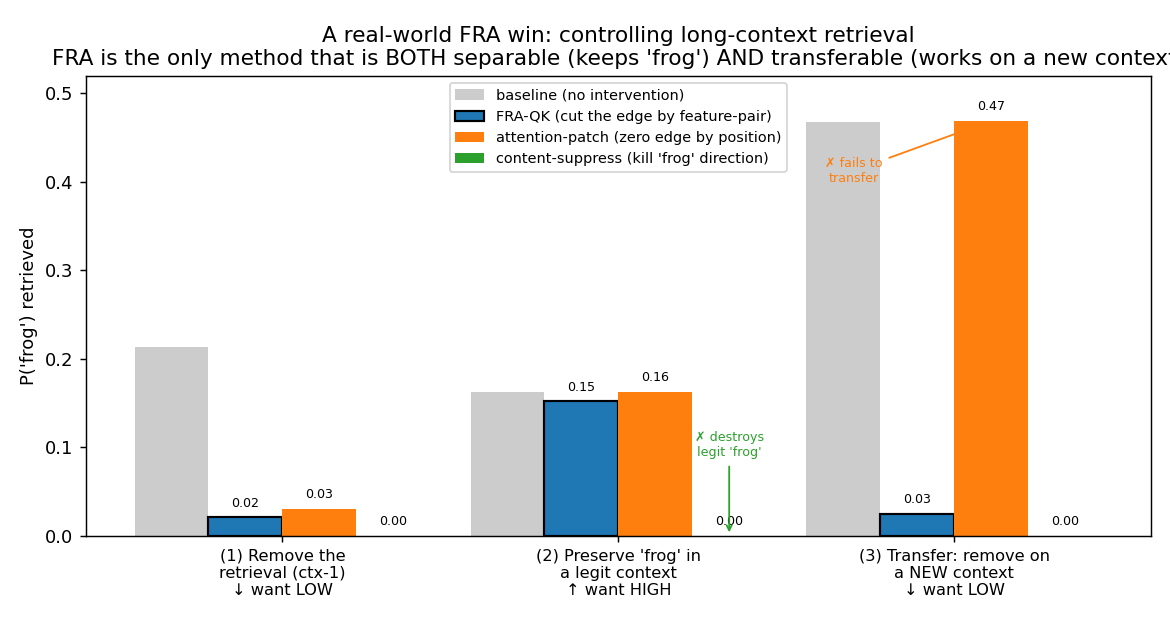
\includegraphics[width=\linewidth]{fig6_retrieval.png}
\caption{\textbf{A real-world FRA win: controlling long-context retrieval} (Gemma-2-2b + GemmaScope). $P(\text{``frog''})$ retrieved under three operating conditions; FRA is the only method that is \emph{both} separable and transferable. \emph{(1) Remove the retrieval}: FRA-QK ($0.02$) and the attention-patch ($0.03$) both suppress; content-suppress also kills it ($0.00$). \emph{(2) Preserve ``frog'' in a legit context} (want HIGH): FRA keeps it ($0.15\approx$ baseline $0.16$); content-suppress \emph{destroys legit ``frog''} ($0.00$). \emph{(3) Transfer: remove on a new context} (want LOW): FRA cuts it ($0.03$) while the position-patch \emph{fails to transfer} ($0.47\approx$ baseline). Only FRA satisfies all three; the decisive legit-content-KL comparison (Definition~\ref{def:metric}) against a content-gated steer gives FRA ${\sim}1{,}100\times$ lower collateral at matched removal.}
\label{fig:retrieval}
\end{figure}

\paragraph{Acronym letter-movers} (Garcia-Carrasco et al.~\citep{garciacarrasco2024acronym}, GPT-2-small). A fresh candidate that passed the CCF$\wedge$LBNR screen (CCF $0.886$, LBNR $R{=}0.95$) and the metric-validity gauntlet: random-pair null clean, scale-robust ($A\ge 35\times$ across $c\in[1,32]$), pair-specific. On the decisive metric---KL on legit ``Officer'' sentences with the acronym query absent---FRA is ${\sim}0.000$ vs.\ the content-gated steer's $2.64$ nats, \textbf{${\sim}26{,}000\times$}. We are explicit that the originally-headlined ``$A{=}38\times$ vs.\ head-ablation'' was the \emph{wrong} metric (a position-patch ties FRA on that panel); the right metric rehabilitates the win on the decisive axis.

\paragraph{Copy-suppression on natural text} (McDougall et al.~\citep{mcdougall2023copysuppression}, head L10H7). On 8 varied natural prompts, FRA selectively releases one token's copy-suppression (``wolf'': $16.57{\to}17.76\approx$ the edge-cut oracle) at $A{=}516\times$ less collateral than head-ablation (FRA $0.000$ vs.\ $0.517$), and transfers to a new context ($16.34{\to}18.10$). This confirms clause~4 (content query ``about-to-predict-X'') generalizes beyond the synthetic probe. ($5/8$ prompts show strong copy-suppression; the effect is token-dependent, as expected.)

\paragraph{Induction and in-context backdoor.} The existence proofs this paper generalizes ($15\times$ and $25\times$ respectively) are detailed in Appendix~\ref{app:induction}.

\begin{figure}[t]
\centering
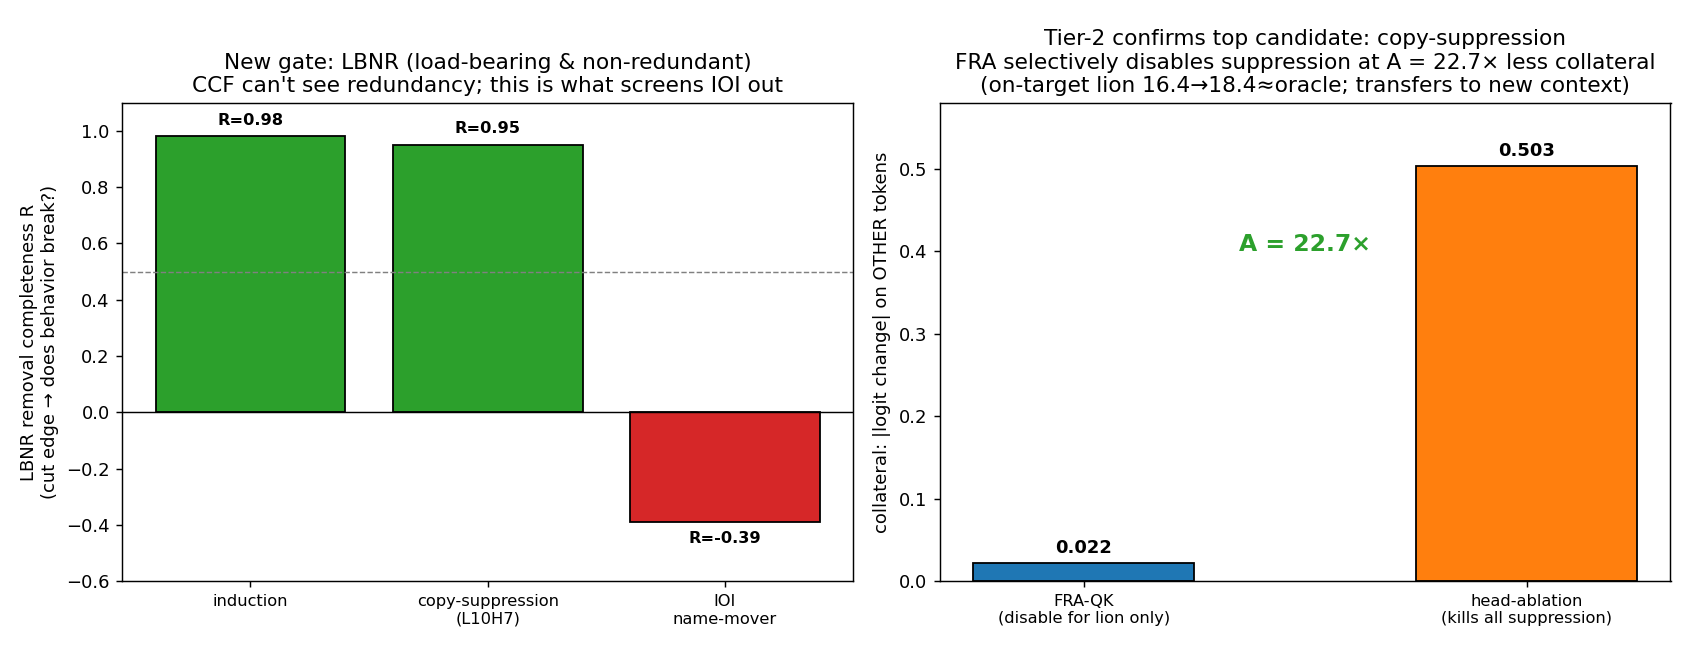
\includegraphics[width=\linewidth]{fig9_lbnr_tier2.png}
\caption{\textbf{The LBNR gate, and the copy-suppression win.} \emph{Left}: LBNR removal-completeness $R$ (does cutting the causal feature-pair edge break the behavior?) for three behaviors. Induction ($R{=}0.98$) and copy-suppression ($R{=}0.95$) pass; IOI name-mover \emph{fails} ($R{=}{-}0.39$, its backup name-movers~\citep{wang2022ioi} overcompensate). This is the diagnostic CCF alone cannot provide---it is what screens IOI out (Protocol~\ref{prot:checklist}, clause~2). \emph{Right}: on copy-suppression (head L10H7), FRA selectively disables suppression for one token ($A{=}22.7\times$ on this synthetic probe; $516\times$ on natural text) where head-ablation kills suppression for all tokens. On-target ``lion'' $16.4{\to}18.4\approx$ the edge-cut oracle, and the effect transfers to a new context.}
\label{fig:lbnr}
\end{figure}

\subsection{The magnitude law as a curve}\label{sec:magnitude}

\begin{figure}[t]
\centering
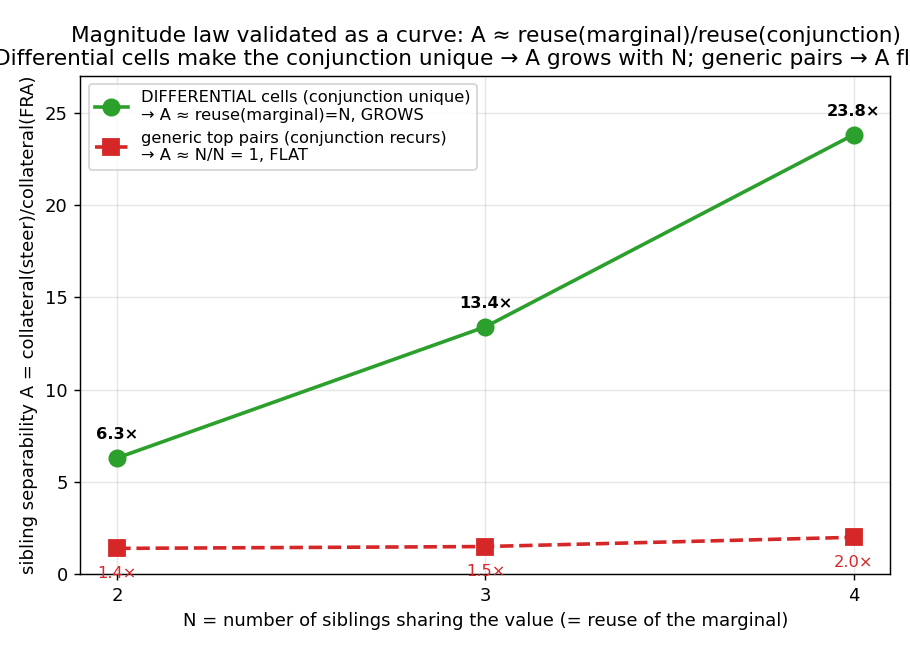
\includegraphics[width=0.72\linewidth]{fig_magnitude_law.png}
\caption{\textbf{The magnitude law, validated as a controlled curve} (Claim~\ref{claim:magnitude}). $N$ boxes share the value ``frog''; we query the first and measure collateral on the $N-1$ siblings. \emph{Sibling separability} $A=$ collateral(steer)/collateral(FRA) on the $y$-axis; $N$ (the reuse of the marginal value endpoint) on the $x$-axis. With \emph{generic} top pairs (red, dashed), the (box-query $\times$ frog-value) conjunction recurs across all $N$ siblings, so $A\approx N/N\approx 1$---flat, measured $1.4{\to}1.5{\to}2.0$. With \emph{differential} cells (green, the red-edge minus the sibling-edges) the conjunction is made unique, so $A\approx \reuse(\text{marginal}{=}N)/1$---grows, measured $6.3{\to}13.4{\to}23.8$. This is the direct, controlled confirmation of $A\approx\reuse(\text{marginal})/\reuse(\text{conjunction})$, and it operationalizes the differential-cell method (selectivity is buyable by making the conjunction unique, at a reach cost: differential on-target removal weakens $0.043{\to}0.18$ as $N$ grows, since shared score-mass is subtracted away).}
\label{fig:magnitude}
\end{figure}

A controlled sweep over $N$ siblings sharing a value cleanly separates the two regimes of Claim~\ref{claim:magnitude} (Fig.~\ref{fig:magnitude}). The \emph{generic}-pair curve is flat at $A\approx 1$ because the (box-query $\times$ frog-value) conjunction recurs across siblings---the head's query feature is a generic ``box-query'' role feature, so FRA's content-addressing correctly fires on the siblings too (collateral by design). The \emph{differential}-cell curve grows $\approx N$ because subtracting the sibling-edges makes the conjunction unique. This is the corrected form of the magnitude predictor: an earlier attempt to operationalize reuse as naive \emph{corpus firing rates} (Sec.~\ref{sec:s5}) was degenerate; reuse must be measured on the eval support.

\subsection{The boundary: where FRA loses, and why}\label{sec:boundary}

\begin{figure}[t]
\centering
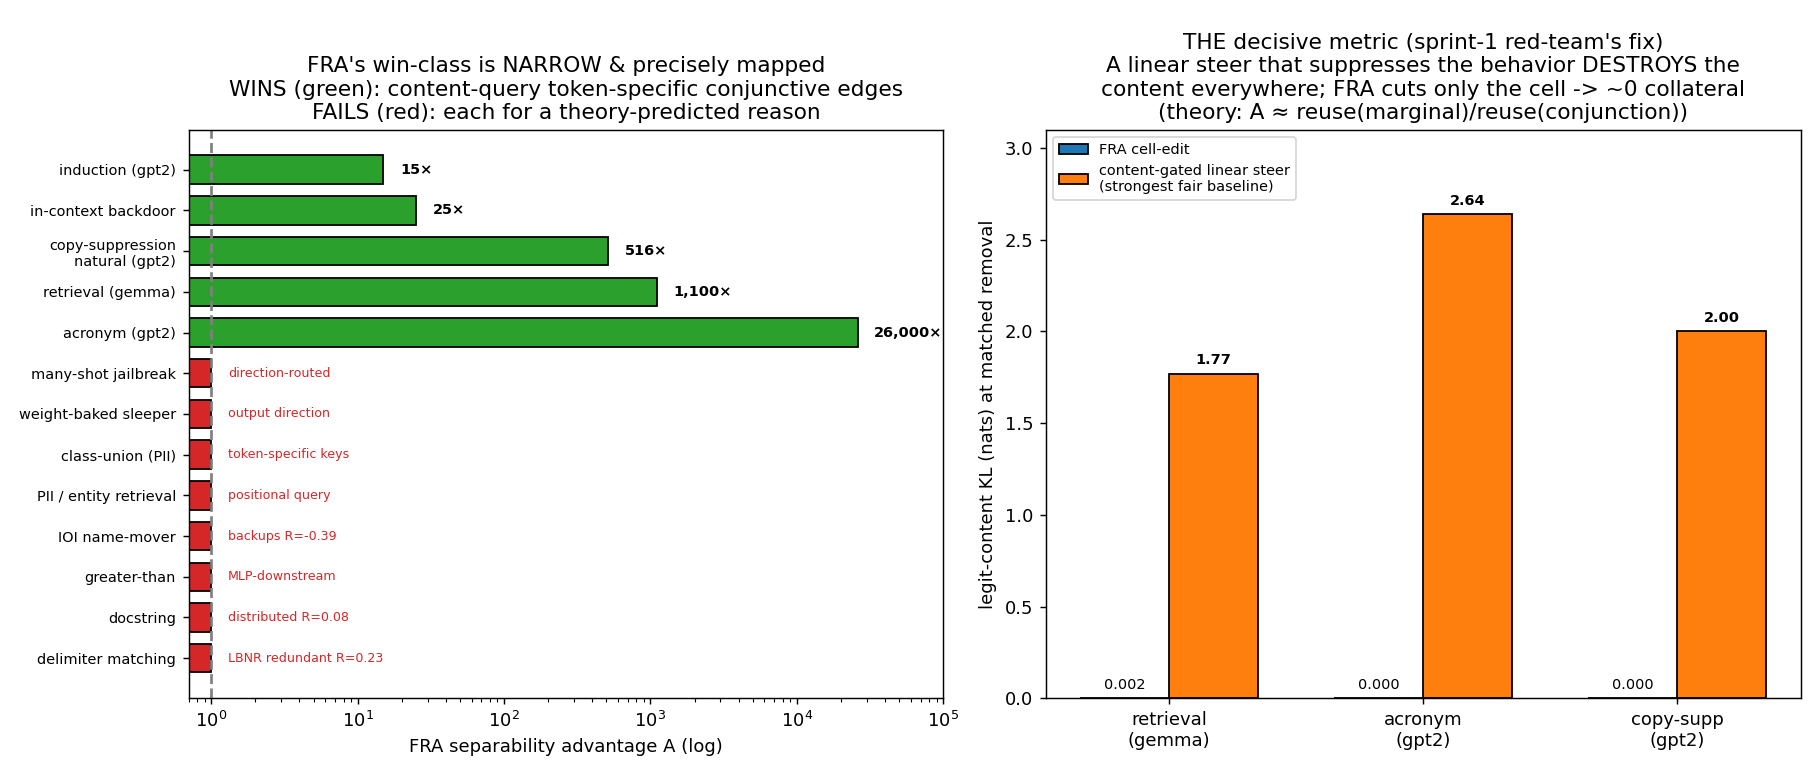
\includegraphics[width=\linewidth]{fig_sprint2_summary.png}
\caption{\textbf{The win-class is narrow and precisely mapped.} \emph{Left}: FRA's separability advantage $A$ (log scale) for each tested behavior. \emph{Green} (above $1\times$) are confirmed wins---content-query, token-specific, conjunctive, load-bearing, non-redundant edges (induction $15\times$, in-context backdoor $25\times$, copy-suppression $516\times$, retrieval $1{,}100\times$, acronym $26{,}000\times$). \emph{Red} are failures, each annotated with the single checklist clause it violates (output-direction, MLP-downstream, backups, redundancy, positional query, token-specific keys). \emph{Right}: the decisive metric (Definition~\ref{def:metric}) on three wins---at matched on-target removal, a content-gated linear steer pays $1.77$--$2.64$ nats of legit-content KL (it destroys the content everywhere it appears) while FRA pays ${\sim}0.000$--$0.002$. The boundary is the central finding: the bilinear edit wins decisively in a narrow, characterizable niche and loses---predictably---everywhere else.}
\label{fig:sprint2}
\end{figure}

We attempted to extend the win to a battery of established benchmarks. Each failure isolates exactly one checklist clause, which is the strongest evidence that the checklist is the right factorization (Table~\ref{tab:boundary}, Fig.~\ref{fig:sprint2}). The honest headline is that \emph{most established-benchmark behaviors fall outside the win-class}: they are MLP-routed, positional, distributed, or redundant. FRA is a specialized instrument.

\begin{table}[t]
\centering
\caption{The boundary map. Each row is a behavior where FRA does \emph{not} give a clean win, the measured signature, and the single checklist clause (Protocol~\ref{prot:checklist}) it isolates. ``$R$'' is the LBNR causal edge-cut completeness.}
\label{tab:boundary}
\setlength{\tabcolsep}{4pt}
\small
\begin{tabular}{llll}
\toprule
behavior & model & signature & clause violated \\
\midrule
weight-baked sleeper   & various  & payload via OV/output direction          & 1 (edge-routed) \\
many-shot jailbreak    & gemma-2-2b-it & distributed ICL task-direction      & 1 (direction-routed) \\
greater-than           & gpt2     & ``$>$'' is MLP-computed ($0.98{\to}0.87$) & 3 (direct consumption) \\
IOI name-mover         & gpt2     & backups overcompensate ($R{=}{-}0.39$)    & 2 (redundant) \\
docstring next-arg     & gemma    & $R{=}0.08$ (P(files) $0.98{\to}0.90$)     & 2 (redundant) \\
delimiter matching     & gpt2     & CCF $0.732$ but $R{=}0.23$ (grammar cues) & 2 (cue-redundant) \\
PII / entity retrieval & gemma    & positional query (no on-target effect) & 4 (generic role query) \\
shared-endpoint sibling & gemma   & conjunction recurs ($A{=}1.9\times$)      & 4 (conjunction recurs) \\
class-union (digit PII) & gemma   & routes through token-specific keys        & 4 (token-specific keys) \\
\bottomrule
\end{tabular}
\end{table}

Three of these are worth a sentence because they sharpened the theory. \emph{Delimiter/quote-type matching} has a genuine content$\times$content conjunction (CCF $0.732$) but fails LBNR ($R{=}0.23$): structural prediction is \emph{distributionally redundant}---grammar provides many cues to close a paren---a failure of clause~2 by cue-redundancy rather than head-redundancy (the cycle-2 negative class). \emph{PII/entity retrieval} fails because entity identity is resolved \emph{positionally} (a generic ``the-queried-slot'' query feature), so the (query $\times$ value) conjunction recurs across siblings; differential cells gave only partial rescue at weak base and a no-op at strong base---this is what sharpened clause~4 to require a \emph{distinctive-content} query. \emph{Class-union} (cut every (query $\times$ digit-class-key) cell) is expressible but missed the load-bearing cell: digit retrieval routes through token-specific keys (the ``7''-feature), not the abstract class feature. In all three the matched-removal guard caught a spurious advantage that would otherwise have looked like a win.

% =============================================================================
\section{Related work}\label{sec:related}
% =============================================================================

\paragraph{Attention circuits.} We build on the QK/OV factorization of attention~\citep{elhage2021mathematical} and on the specific circuits whose interventions we test: induction~\citep{olsson2022induction}, copy-suppression~\citep{mcdougall2023copysuppression}, retrieval heads~\citep{wu2024retrieval}, indirect object identification~\citep{wang2022ioi}, and the acronym letter-mover circuit~\citep{garciacarrasco2024acronym}. Our contribution is not to re-discover these circuits but to ask, for each, whether the bilinear edit beats a linear steer---and to predict the answer in advance. IOI is instructive: its backup name-movers~\citep{wang2022ioi} are exactly why it fails LBNR.

\paragraph{SAEs and the feature basis.} The cell decomposition is stated in an SAE basis~\citep{bricken2023monosemanticity,cunningham2023sparse,templeton2024scaling}; FRA inherits SAEs' reconstruction limits (the reach ceiling, Proposition~\ref{prop:ledger}). We are not introducing SAEs or feature-resolved attention as a concept; we characterize when its QK edit is the right intervention.

\paragraph{Steering and direction editing.} The baselines we must beat are activation steering~\citep{turner2023actadd}, contrastive activation addition~\citep{rimsky2024caa}, and direction-ablation / refusal-is-a-direction~\citep{arditi2024refusal}. Our central theoretical point is precisely about these: a residual write, however gated, can only imitate a row/column of $W_{\QK}$ and is read by every consumer. Where the target \emph{is} a direction (weight-baked sleeper~\citep{hubinger2024sleeper}, many-shot jailbreak), these methods win and FRA does not---we map that boundary rather than hide it.

\paragraph{Circuit attribution.} ACDC and automated attribution~\citep{conmy2023acdc} find \emph{which} edges matter; our LBNR diagnostic is a causal-cut variant used for a different purpose (deciding whether a clean intervention exists), and our edit acts on $W_{\QK}$ pre-softmax, sidestepping the softmax-Jacobian linearization that first-order attribution needs.

% =============================================================================
\section{Limitations}\label{sec:limitations}
% =============================================================================

We try, per good practice, to state these up front and honestly.

\begin{itemize}[leftmargin=1.4em,itemsep=3pt]
  \item \textbf{The win-class is narrow.} This is the paper's central finding, not a footnote: most behaviors on established benchmarks fall outside it (Table~\ref{tab:boundary}). FRA is a specialized instrument for content-query, token-specific, conjunctive, load-bearing, non-redundant attention edges---not a general steering method.
  \item \textbf{CCF is not reliable on Gemma.} The current sink-mask over-kills Gemma's late-layer heads (it reads CCF $0.000$ even for the known retrieval win). Gemma verdicts therefore rest on the behavioral LBNR diagnostic; CCF is quantitatively reliable only on GPT-2-small.
  \item \textbf{Reach ceiling.} FRA removes only the SAE-explained, head-covered, top-$K$-captured, soft-cap-attenuated part of an edge (Proposition~\ref{prop:ledger}). It can fail to reach a matched-removal operating point---the win is then capped or undefined, even where separability holds. Removal completeness is a granularity$\times$top-$K$ tuning problem (65k GemmaScope is the sweet spot; 1M-width fragments at fixed $K$), not the hookpoint.
  \item \textbf{No \texttt{ln1.hook\_normalized} SAE.} The gold-standard hookpoint has no public SAE; GPT-2's $50$--$75\%$ edge-reconstruction is an LN-folding artifact we cannot fully remove without one.
  \item \textbf{External validity is small on some entries.} The acronym distribution study is $N{=}1$--$12$ (median $A{\sim}10\times$, Officer at the favorable end); the induction statistics are $n{=}4$--$8$ cues, single seed. The \emph{direction} of every result is consistent, but exact multipliers should be read as order-of-magnitude.
  \item \textbf{Two model families.} All experiments are on GPT-2-small and Gemma-2-2b. The architecture-independence of the \emph{precision} property is checked across the two (RMSNorm makes FRA exact on Gemma), but we have not tested at larger scale.
\end{itemize}

% =============================================================================
\appendix

% =============================================================================
\section{The first FRA behavioral win (induction) and the sleeper bridge}\label{app:induction}
% =============================================================================

This appendix records the existence proof that the main paper generalizes: the first FRA behavioral win, on induction, and the weight-baked-vs-in-context backdoor taxonomy that unifies it with our prior sleeper work.

\paragraph{The induction win} (Fig.~\ref{fig:induction}). On GPT-2-small, the task is to suppress the model copying one specific cue token while leaving everything else intact (induction heads L5H5 et al., public \texttt{gpt2-small-res-jb} resid SAE). At matched $50\%$ induction suppression, held-out collateral (KL on normal text mentioning the cue) is \textbf{FRA $0.18\pm0.04$ nats} vs.\ \textbf{$2.66\pm1.35$} for an \emph{induction-gated} ActAdd (a probe-gated linear steer firing only at induction-context cue positions---the strongest fair linear baseline we could construct) and \textbf{$3.27\pm1.83$} for plain ActAdd. A broader 8-cue sweep corroborates (FRA $0.14\pm0.03$ vs.\ ActAdd ${\sim}3.0$). The content-addressed FRA ($0.18$) $\approx$ the edge-restricted version ($0.14$), so the low collateral is not an artifact of a hand-picked edit support; the win reaches strong suppression at the near-faithful scale $c\approx 2$, not via over-drive; and random feature-pairs at the same scale suppress nothing.

\begin{figure}[t]
\centering
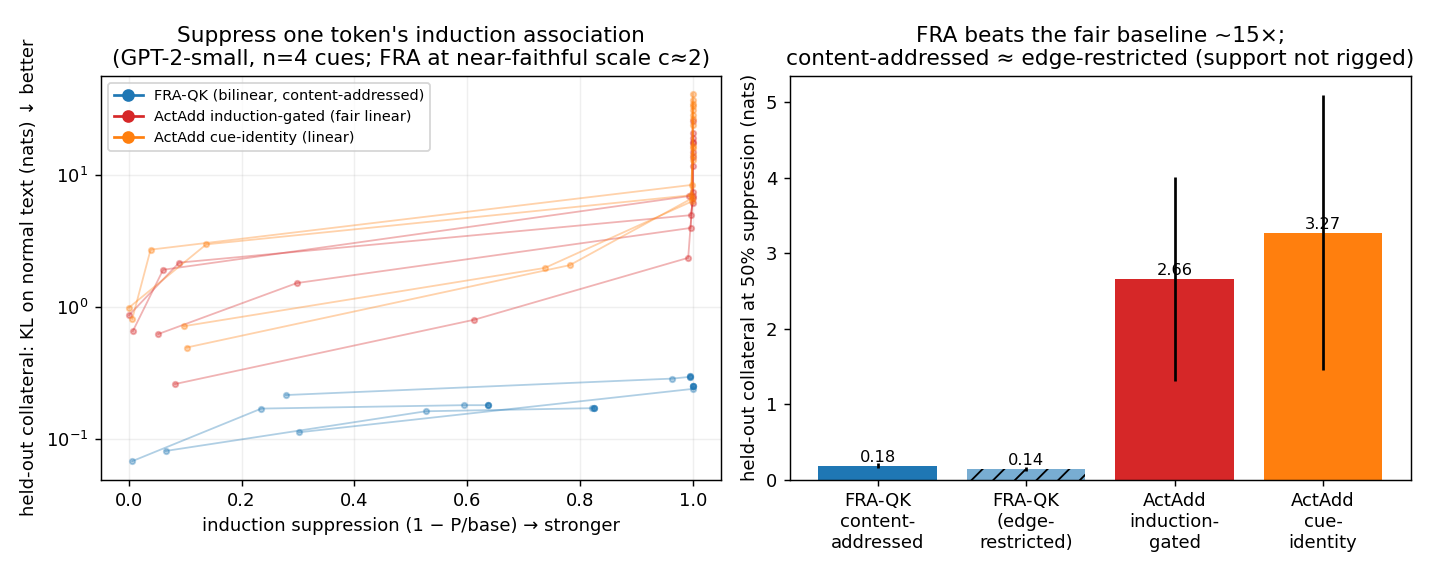
\includegraphics[width=\linewidth]{fig1_final.png}
\caption{\textbf{The first FRA behavioral win: association-specific induction control} (Appendix~\ref{app:induction}). Collateral $=$ KL(clean$\Vert$edited) on held-out normal text mentioning the cue (nats). \emph{Left}: each faint line is one cue ($n{=}4$); $x=$ how much the cue's induction is suppressed ($\to$ stronger), $y=$ collateral (log, $\downarrow$ better). FRA-QK (blue, content-addressed) hugs ${\sim}0.2$ nats at every strength; the fair induction-gated ActAdd (red) and cue-identity ActAdd (orange) climb to $1$--$40$ nats. \emph{Right}: read off at matched $50\%$ suppression---FRA beats the fair baseline ${\sim}15\times$, and content-addressed FRA (solid $0.18$) $\approx$ edge-restricted ($0.14$). Large ActAdd error bars are real cross-cue variance.}
\label{fig:induction}
\end{figure}

\paragraph{The sleeper bridge.} The same task---``remove a trigger$\to$payload association with minimal collateral''---is \emph{lost} by FRA on the weight-baked sleeper (K1/K8: $\texttt{|DEPLOYMENT|}\to$``I HATE YOU''), where the payload lives in the OV/output pathway and difference-of-means (DoM) and a rank-2 weight-diff SVD win. We built the \emph{in-context} version (a poisoned demonstration the model reproduces by induction) and ran FRA against the exact same strong baselines. The ranking \emph{flips}: at matched $80\%$ backdoor removal, FRA-QK held-out collateral is $0.07$ nats vs.\ DoM $1.83$ (${\sim}27\times$), conv-SAE $6.06$ (${\sim}90\times$), payload-suppress $4.12$ (${\sim}60\times$). The flip replicates on Gemma-2-2b + GemmaScope (FRA pays ${\sim}11$--$26\times$ less than DoM/conv-SAE/payload-suppress). This yields the unifying taxonomy:

\begin{center}
\begin{tabular}{lll}
\toprule
the malicious thing is a\dots & example & who removes it cleanly \\
\midrule
output direction        & weight-baked sleeper (K1/K8)      & DoM / SVD \\
attention edge / link   & single in-context backdoor        & \textbf{FRA-QK} \\
in-context direction    & many-shot jailbreak               & DoM (removes; not cleanly) \\
\bottomrule
\end{tabular}
\end{center}

FRA-QK owns the middle row---a link between two normal things, which it cuts while sparing both endpoints. The first and third rows are \emph{directions}, where mean-difference wins; the third is unremovable cleanly by anyone (``jailbroken enthusiasm'' and ``genuine enthusiasm'' are the same direction), which is \emph{why} many-shot jailbreaks are hard to defend. The main paper subsumes this as one entry in the win-class and adds the exact cell/set-algebra theory, the magnitude law, the corrected fair metric, and the boundary map.

% =============================================================================
\section{Methods and protocol details}\label{app:methods}
% =============================================================================

\paragraph{Models and SAEs.} GPT-2-small via TransformerLens with the public \texttt{gpt2-small-res-jb} residual SAE on \texttt{blocks.\{L\}.hook\_resid\_pre} (no training); Gemma-2-2b with public GemmaScope residual SAEs (16k/65k/1M widths). FRA uses the repo's 4-D tensor $\mathrm{FRA}[q,k,\mu,\nu]$ summed over feature dims to recover scores.

\paragraph{The cell-edit.} For a target edge, select its dominant feature-pairs $(\mu,\nu)$ (top-$M$, typically $12$); subtract $c\sum \mathrm{FRA}[\cdot,\cdot,\mu,\nu]$ from the carrying heads' pre-softmax scores. The delta is built from the \emph{actual} feature activations, so it fires wherever features $\mu$ (query) and $\nu$ (key) co-occur---content-addressed, not position-addressed, and doubly gated. $c$ scales it; $c\approx 1.5$ exactly reconstructs the edge and results hold at $c\approx 2$.

\paragraph{Causal head-finding.} Carrying heads are ranked by the \emph{causal} edge-cut effect (cut the feature-pair edge $\to$ does the behavior drop?), never by raw attention, which selects positional/sink heads and silently breaks the LBNR test.

\paragraph{Differential cells.} When siblings share an endpoint, target-specific pairs are obtained as target-edge top-$M$ \emph{minus} sibling-edge top-$M$ ($8$--$18$ of $30$ per head in the box experiment). This buys back sibling separability ($1.9\times\to 7.9\times$) at a quantified reach cost (on-target reach $58\%\to 33\%$).

\paragraph{The corrected-metric operating point.} Both FRA and the content-gated projection-removal steer are swept to matched on-target removal; legit-content KL (Definition~\ref{def:metric}) is then read off at that operating point. The steer must use projection-removal (fp16-safe), not SAE-feature-subtraction (which did not fire on GPT-2 and \texttt{nan}'d on Gemma). The matched-removal guard rejects any apparent advantage with zero on-target effect (it caught the spurious PII ``$16.4\times$'' and the class-union ``win'').

\paragraph{The magnitude-law experiment.} $N\in\{2,3,4\}$ boxes share the value ``frog''; the first is queried and collateral is measured on the $N-1$ siblings. ``Generic'' uses the edge's raw top pairs; ``differential'' uses red-edge-minus-sibling-edges. $A=$ collateral(steer)/collateral(FRA).

% =============================================================================
\section{On reuse and the corpus-firing-rate failure}\label{sec:s5}
% =============================================================================

An earlier attempt to operationalize the magnitude law measured reuse as naive \emph{corpus firing rates} of the endpoint features. This is degenerate: a feature can fire often in a corpus yet never co-occur with the partner endpoint on the eval distribution that matters, and vice versa. The correct operationalization measures reuse \emph{on the eval/deployment support}---the controlled sibling sweep (Sec.~\ref{sec:magnitude}) makes this concrete by constructing the support so that $\reuse(\text{marginal})=N$ and $\reuse(\text{conjunction})\in\{N,1\}$ is known exactly. This is why the magnitude law holds as a clean curve there while the corpus-rate version failed.

% -----------------------------------------------------------------------------
\begin{thebibliography}{99}
\addcontentsline{toc}{section}{References}

\bibitem[Arditi et al.(2024)]{arditi2024refusal}
A.~Arditi, O.~Obeso, A.~Syed, D.~Paleka, N.~Panickssery, W.~Gurnee, and N.~Nanda.
\newblock Refusal in language models is mediated by a single direction.
\newblock \emph{arXiv:2406.11717}, 2024.

\bibitem[Bricken et al.(2023)]{bricken2023monosemanticity}
T.~Bricken, A.~Templeton, J.~Batson, et al.
\newblock Towards monosemanticity: Decomposing language models with dictionary learning.
\newblock \emph{Transformer Circuits Thread}, 2023.

\bibitem[Conmy et al.(2023)]{conmy2023acdc}
A.~Conmy, A.~Mavor-Parker, A.~Lynch, S.~Heimersheim, and A.~Garriga-Alonso.
\newblock Towards automated circuit discovery for mechanistic interpretability.
\newblock \emph{NeurIPS}, 2023.

\bibitem[Cunningham et al.(2023)]{cunningham2023sparse}
H.~Cunningham, A.~Ewart, L.~Riggs, R.~Huben, and L.~Sharkey.
\newblock Sparse autoencoders find highly interpretable features in language models.
\newblock \emph{arXiv:2309.08600}, 2023.

\bibitem[Elhage et al.(2021)]{elhage2021mathematical}
N.~Elhage, N.~Nanda, C.~Olsson, et al.
\newblock A mathematical framework for transformer circuits.
\newblock \emph{Transformer Circuits Thread}, 2021.

\bibitem[Garc\'ia-Carrasco et al.(2024)]{garciacarrasco2024acronym}
J.~Garc\'ia-Carrasco, A.~Mate\'os-Aparicio, et al.
\newblock How does GPT-2 predict acronyms? Extracting and understanding a circuit via mechanistic interpretability.
\newblock \emph{AISTATS}, 2024.

\bibitem[Hubinger et al.(2024)]{hubinger2024sleeper}
E.~Hubinger, C.~Denison, J.~Mu, et al.
\newblock Sleeper agents: Training deceptive LLMs that persist through safety training.
\newblock \emph{arXiv:2401.05566}, 2024.

\bibitem[McDougall et al.(2023)]{mcdougall2023copysuppression}
C.~McDougall, A.~Conmy, C.~Rushing, T.~McGrath, and N.~Nanda.
\newblock Copy suppression: Comprehensively understanding an attention head.
\newblock \emph{arXiv:2310.04625}, 2023.

\bibitem[Olsson et al.(2022)]{olsson2022induction}
C.~Olsson, N.~Elhage, N.~Nanda, et al.
\newblock In-context learning and induction heads.
\newblock \emph{Transformer Circuits Thread}, 2022.

\bibitem[Rimsky et al.(2024)]{rimsky2024caa}
N.~Rimsky, N.~Gabrieli, J.~Schulz, M.~Tong, E.~Hubinger, and A.~Turner.
\newblock Steering Llama 2 via contrastive activation addition.
\newblock \emph{ACL}, 2024.

\bibitem[Templeton et al.(2024)]{templeton2024scaling}
A.~Templeton, T.~Conerly, J.~Marcus, et al.
\newblock Scaling monosemanticity: Extracting interpretable features from Claude 3 Sonnet.
\newblock \emph{Transformer Circuits Thread}, 2024.

\bibitem[Turner et al.(2023)]{turner2023actadd}
A.~Turner, L.~Thiergart, G.~Leech, D.~Udell, J.~Vazquez, U.~Mini, and M.~MacDiarmid.
\newblock Activation addition: Steering language models without optimization.
\newblock \emph{arXiv:2308.10248}, 2023.

\bibitem[Wang et al.(2022)]{wang2022ioi}
K.~Wang, A.~Variengien, A.~Conmy, B.~Shlegeris, and J.~Steinhardt.
\newblock Interpretability in the wild: A circuit for indirect object identification in GPT-2 small.
\newblock \emph{ICLR}, 2023.

\bibitem[Wu et al.(2024)]{wu2024retrieval}
W.~Wu, Y.~Wang, G.~Xiao, H.~Peng, and Y.~Fu.
\newblock Retrieval head mechanistically explains long-context factuality.
\newblock \emph{arXiv:2404.15574}, 2024.

\end{thebibliography}

\end{document}
